% 
% Permission is granted to copy, distribute and/or modify this document
% under the terms of the GNU Free Documentation License, Version 1.2
% or any later version published by the Free Software Foundation;
% with no Invariant Sections, no Front-Cover Texts, and no Back-Cover
% Texts.  A copy of the license is included in the section entitled "GNU
% Free Documentation License".

\documentclass[11pt]{article}

\usepackage{OTPMML_Documentation}
\usepackage{Math_Notations}

\makeindex

\begin{document}

\thispagestyle{empty}

% 
% Permission is granted to copy, distribute and/or modify this document
% under the terms of the GNU Free Documentation License, Version 1.2
% or any later version published by the Free Software Foundation;
% with no Invariant Sections, no Front-Cover Texts, and no Back-Cover
% Texts.  A copy of the license is included in the section entitled "GNU
% Free Documentation License".
\vspace*{2cm}

\begin{center}
  {\huge \bf Documentation of the OTPMML module}
  \input{GenericInformation.tex}
\end{center}



\newpage
% Permission is granted to copy, distribute and/or modify this document
% under the terms of the GNU Free Documentation License, Version 1.2
% or any later version published by the Free Software Foundation;
% with no Invariant Sections, no Front-Cover Texts, and no Back-Cover
% Texts.  A copy of the license is included in the section entitled "GNU
% Free Documentation License".
% Copyright 2014 EDF
%  

\vspace{0.5in}
\begin{center}
\vspace{0.3in}
\emph{\fontshape{sc} Abstract}
\vspace{0.5in}
\end{center}

The purpose of this document is to present the OTPMML module.

This document is organized according to the OpenTURNS documentation :
\begin{itemize}
\item \itshape{Architecture Guide} gives UML diagrams of all implemented classes,
\item \itshape{Reference Guide} gives some theoretical basis,
\item \itshape{Use cases Guide} details scripts in Python (the Textual Interface language of OpenTURNS) and helps to learn as quickly as possible the manipulation of the \textit{otpmml} module,
\item \itshape{User Manual} details the \textit{otpmml} objects and give the list of their methods,
\item \itshape{Validation Guide} which provides use cases to validate the \textit{otpmml} module.
\end{itemize}

\tableofcontents
\newpage
% Permission is granted to copy, distribute and/or modify this document
% under the terms of the GNU Free Documentation License, Version 1.2
% or any later version published by the Free Software Foundation;
% with no Invariant Sections, no Front-Cover Texts, and no Back-Cover
% Texts.  A copy of the license is included in the section entitled "GNU
% Free Documentation License".
% Copyright 2014 EDF
%

%%%%%%%%%%%%%%%%%%%%%%%%%%%%%%%%%%%%%%%%%%%%%%%%%%%%%%%%%%%%%%%%%%%%%%%%%%%%%%%%%%%%%%%%%%
\section{Architecture guide}

This document makes up the general specification design for the architecture of the OTPMML module.

\subsection{DAT}

\begin{figure}[htb]
  \begin{center}
    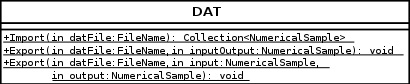
\includegraphics[scale=0.8]{DAT.png}
    \caption{DAT class}\label{fig:archi:DAT}
  \end{center}
\end{figure}

The \texttt{DAT} class is a utility class to import and export Uranie \texttt{.dat} files.  It contains only static methods.

\subsection{NeuralNetwork}

\begin{figure}[htb]
  \begin{center}
    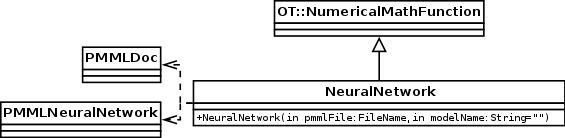
\includegraphics[scale=0.8]{NeuralNetwork.png}
    \caption{NeuralNetwork class}\label{fig:archi:NeuralNetwork}
  \end{center}
\end{figure}

The \texttt{NeuralNetwork} class inherits from \texttt{NumericalMathFunction}.
It uses \texttt{PMMLDoc} and \texttt{PMMLNeuralNetwork} internal classes to parse \texttt{.pmml} files written by Uranie.

\subsection{RegressionModel}

\begin{figure}[htb]
  \begin{center}
    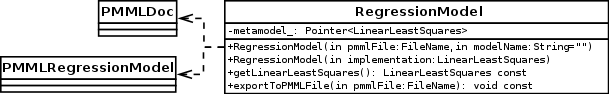
\includegraphics[scale=0.8]{RegressionModel.png}
    \caption{RegressionModel class}\label{fig:archi:RegressionModel}
  \end{center}
\end{figure}

The \texttt{RegressionModel} class is a wrapper around \texttt{RegressionModel} XML elements found in \texttt{.pmml} files.
It uses \texttt{PMMLDoc} and \texttt{PMMLRegressionModel} internal classes.

\subsection{PMML Internal Classes}

\subsubsection{PMMLDoc}

\begin{figure}[htb]
  \begin{center}
    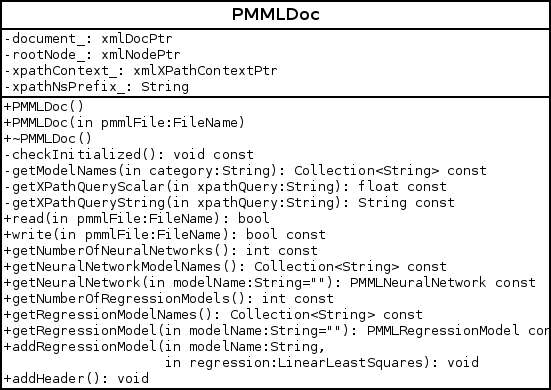
\includegraphics[scale=0.8]{PMMLDoc.png}
    \caption{PMMLDoc class}\label{fig:archi:PMMLDoc}
  \end{center}
\end{figure}

The \texttt{PMMLDoc} class reads an XML file (in the PMML 3.0 format, which is
the format used by Uranie), and provides several methods used by
\texttt{PMMLNeuralNetwork} and \texttt{PMMLRegressionModel} classes.
It internally uses LibXML2 library to handle XML data; this library must be initialized
before parsing XML data, and memory must be explicitly deallocated when its job is over.
For this reason, it had been decided to not expose \texttt{PMMLDoc} to the Python interface.
Calls to \texttt{xmlInitParser} and \texttt{xmlCleanupParser} are performed by higher-level
classes \texttt{NeuralNetwork} and \texttt{RegressionModel}.

XPath is used extensively to extract informations from XML data; two methods,
\texttt{getXPathQueryScalar} and \texttt{getXPathQueryString}, are provided for
simple usages.  \texttt{PMMLNeuralNetwork} and \texttt{PMMLRegressionModel} classes
are declared \texttt{friend} so that they can use these methods.

The \verb+xpathContext_+ member stores the current XPath context, and is modified by
\texttt{setXPathContext} methods of \texttt{PMMLNeuralNetwork} and \texttt{PMMLRegressionModel} classes
to point to their respective XML elements.

There are some caveats with XML namespaces when using XPath.  In order to parse XML files with or
without namespaces, an \verb+xpathNsPrefix_+ member has been added.

\paragraph{Note:}
In \texttt{addRegressionModel}, the \texttt{LinearLeastSquares} argument cannot be passed as a
const reference due to a bug which had been fixed only in OpenTURNS 1.5.

\subsubsection{PMMLRegressionModel}

\begin{figure}[htb]
  \begin{center}
    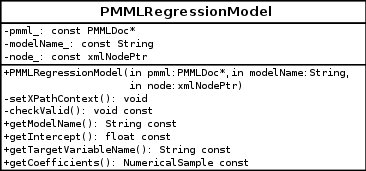
\includegraphics[scale=0.7]{PMMLRegressionModel.png}
    \caption{PMMLRegressionModel class}\label{fig:archi:PMMLRegressionModel}
  \end{center}
\end{figure}

The \texttt{PMMLRegressionModel} class is straightforward.  The \texttt{checkValid} private method ensures that
this regression model can be mapped to a \texttt{LinearLeastSquares} instance.  The following checks are performed:
\begin{itemize}
\setlength{\itemsep}{0pt}
\item \texttt{modelType} attribute, if present, must be equal to \texttt{linearRegression}
\item \texttt{functionName} attribute must be equal to \texttt{regression}
\item \texttt{normalizationMethod} attribute must be equal to \texttt{none}
\item there must be only one \texttt{RegressionTable} child element
\item this \texttt{RegressionTable} must contain only \texttt{NumericPredictor} children and not \texttt{CategoricalPredictor}
\item \texttt{exponent} attributes of \texttt{NumericPredictor} must be equal to 1
\end{itemize}

\subsubsection{PMMLNeuralNetwork}

\begin{figure}[htb]
  \begin{center}
    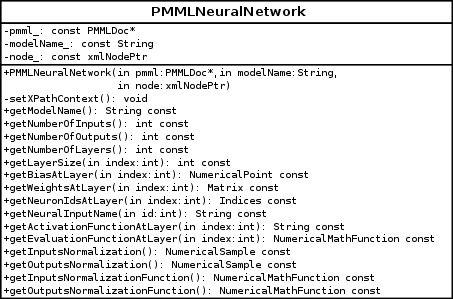
\includegraphics[scale=0.7]{PMMLNeuralNetwork.png}
    \caption{PMMLNeuralNetwork class}\label{fig:archi:PMMLNeuralNetwork}
  \end{center}
\end{figure}

The \texttt{PMMLNeuralNetwork} class parses XML data and provides accessor methods which are used by \texttt{NeuralNetwork}.
Most functions could be private, they are public only to help testing and debugging.

Any valid \texttt{NeuralNetwork} XML element should be supported.  There may be any number of hidden layers, neural layers may have any number of neurons, layers may be sparse, all known activation functions are supported.  The only restriction is with normalization of inputs and outputs, piecewise normalization is not supported.  This should not be a problem since Uranie stores PMML files with this format.

\paragraph{Note:}
\texttt{NumericalMathFunction} is built from string formulas.  In order to preserve accuracy, 20 digits are used.  The drawback is that pretty-printing looks uglier than with less digits.

\newpage
% 
% Permission is granted to copy, distribute and/or modify this document
% under the terms of the GNU Free Documentation License, Version 1.2
% or any later version published by the Free Software Foundation;
% with no Invariant Sections, no Front-Cover Texts, and no Back-Cover
% Texts.  A copy of the license is included in the section entitled "GNU
% Free Documentation License".




%%%%%%%%%%%%%%%%%%%%%%%%%%%%%%%%%%%%%%%%%%%%%%%%%%%%%%%%%%%%%%%%%%%%%%%%%%%%%%%%%%%%%%%%%% 
\section{Reference Guide}

The OTPMML library provides an interface to the \texttt{URANIE} platform.  In particular, it can:
\begin{itemize}
\item read artificial neural networks generated by \texttt{URANIE} and transform them into a \texttt{NumericalMathFunction} which can be used by OpenTURNS algorithms
\item read inputs and outputs generated by \texttt{URANIE}
\item write inputs and outputs in \texttt{URANIE} format
\item convert regression model generated by \texttt{URANIE} into \texttt{LinearLeastSquares} instances, in both directions
\end{itemize}

\subsection{Neural network}

\MathematicalDescription{
\underline{\textbf{Goal}}\\
The aim is to build an artificial neural network (often called neural network) function issued from the \texttt{URANIE} platform.
This mathematical model is inspired by biological neural networks. \\


\underline{\textbf{Principles}}\\
A single-layer perceptron is given by $n+1$ data and an activation function:
\begin{itemize}
 \item $w\in\mathbb{R}^n$ a vector of weights;
 \item $\theta$ a real number, called bias;
 \item $\phi$: activation function, i.e. the rule. Formally, $\phi:\mathbb{R} \rightarrow [0,1]$
\end{itemize}
The expression of neural network model, evaluated on the point of interest $x\in \mathbb{R}^n$, is given by:
\begin{align}
\mathcal{M}(x) & = \phi(w^Tx-\theta)\\
               & = \phi\left(\sum_{i=1}^{n} w_i x_i-\theta\right)
\end{align}
Usually, the notation adopted is:
\begin{equation}
\mathcal{M}(x) = \phi\left(\sum_{i=1}^{n+1} w_i x_i\right)
\end{equation}
with $w_{n+1}=\theta, x_{n+1}=-1$. This model is referred as single layer and described hereafter.
\begin{center}
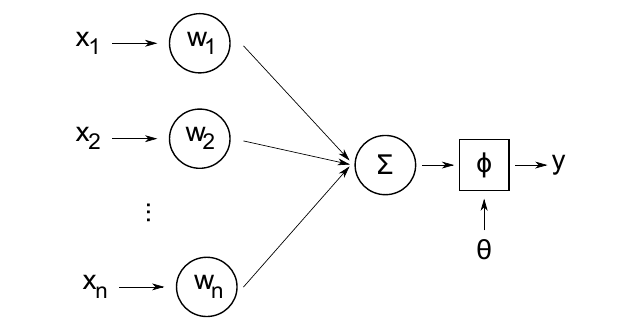
\includegraphics[scale=0.4]{perceptron.png}
% \label{single_layer}
% \caption{A single layer perceptron}
\end{center}

The activation function has to be fixed. The Heaviside function is commonly used and defined by:
\[H(x)= \begin{cases}
      0 & x< 0 \\
      1 & x\geq 0 
   \end{cases}
\]
This function is however discontinuous and thus implies more complexity during the learning step.\\
In machine learning, several functions are commonly used:
\begin{itemize}
 \item The logistic function:
$\displaystyle \sigma(x) = \frac{1}{1+e^{-x}}$
 \item The hyperbolic tangent function:
$\displaystyle \text{tanh}(x) = \frac{e^x - e^{-x}}{e^x+e^{-x}}$
\end{itemize}
These functions are implemented in the module.

A multi-layer perceptron consists of multiple layers of perceptrons, each neuron in a layer being connected to neurons of the previous layer.
Each layer also contains an activation function (which has the same properties as with single-layer perceptrons) and a bias.  The most commonly
used multi-layer perceptron is the 2-layer perceptron:
\begin{center}
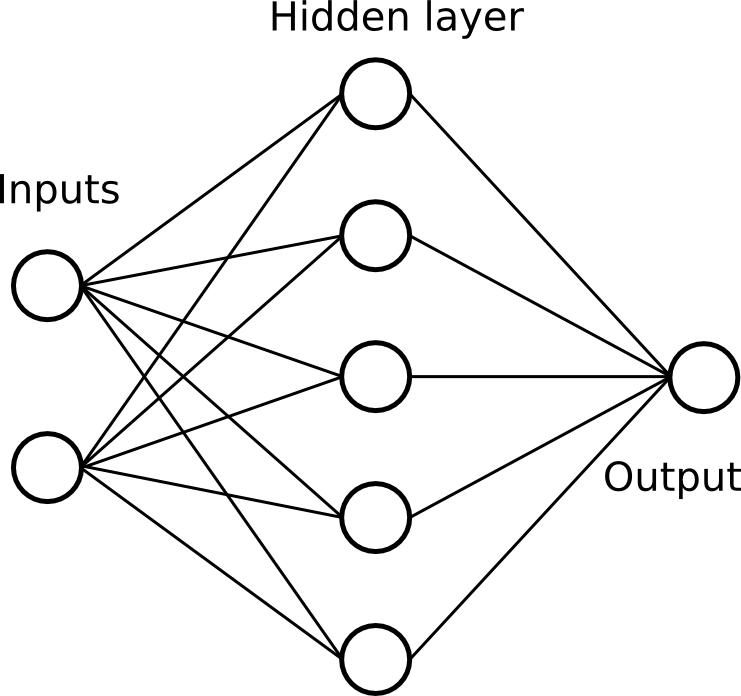
\includegraphics[scale=0.3]{single_layer.png}
\end{center}

If we note $(w,\theta,\phi)$ (resp. $(w^H,\theta^H,\phi^H)$) weights, bias and activation function of the output layer (resp. hidden layer), then
the expression of this neural network model, evaluated on the point of interest $x\in \mathbb{R}^n$, is given by:
\begin{eqnarray*}
\mathcal{M}(x) &=& \phi\left( \sum_{j=1}^M{w_j \mathcal{M}^H_j(x) - \theta} \right) \\
     &=& \phi\left[ \sum_{j=1}^M{w_j \phi^H\left(\sum_{k=1}^{M^H}{w^H_k x_k - \theta^H}\right) - \theta} \right] \\
\end{eqnarray*}

This can be generalized to any number of layers, but in practice a single hidden layer is sufficient.
}

{
% Autres notations et appellations
}

\Methodology{
This method is aimed at building a response surface prior to tackling Step C “Uncertainty Propagation”.
It requires an experimental design together with the corresponding model evaluations.
}
{

\vspace{1mm}

\begin{itemize}
\item Christopher M. Bishop 1995, ``Neural Networks for Pattern Recognition'', Oxford University Press, Inc, New York.
\end{itemize}
}

\subsection{Regression model}
\MathematicalDescription{
\underline{\textbf{Goal}}\\

The objectif is to evaluate a linear model regression issued from the \texttt{URANIE} platform.\\ 
  
\underline{\textbf{Principles}}\\

One considers global approximations of the model response using a polynomial of degree one:
\begin{align*}
  y \, \, \approx \, \, \widehat{h}(\underline{x}) \, \, = \, \, a_0 \, + \,  \sum_{i=1}^{n_{X}} \; a_{i} \; x_i
\end{align*}
where $(a_j  \, , \, j=0,\dots,n_X)$ is a set of unknown coefficients. \\

Several techniques are used to estimate the coefficients of the model.\\
In the propagation context, an experimental design $\underline{\mathcal{X}} =(x^{(1)},\dots,x^{(N)})$, i.e. a set of realizations of input parameters is required, as well 
as the corresponding model evaluations $\underline{\mathcal{Y}} =(y^{(1)},\dots,y^{(N)})$. Thus the coefficients $a_j$ may be computed using a least squares regression approach. \\

The following minimization problem has to be solved:
\begin{align*}
  \mbox{Find} \quad \widehat{\underline{a}} \quad \mbox{that minimizes} \quad \mathcal{J}(\underline{a}) \, \, = \, \, \sum_{i=1}^N \; \left( y^{(i)} \; - \; a_0 - \sum_{j=1}^{n_{X}} a_j \underline{x_{j}}^{(i)} \right)^2
\end{align*}

A necessary condition is that the size $N$ of the experimental design is not less than the number $n_{X}+1$ of coefficients to estimate. \\
%Over techniques may be investigated
}

{
% Autres notations et appellations
}

\Methodology{
Within the global methodology, the method is used to assess the accuracy of a polynomial response surface
of a model output prior to tackling the step C: <<Uncertainty propagation>>.

}
{
\vspace{1mm}
\begin{itemize}
\item {\AA}. Bjorck, 1996, ``Numerical methods for least squares problems'', SIAM Press, Philadelphia, PA.
\end{itemize}

}

\newpage
% 
% Permission is granted to copy, distribute and/or modify this document
% under the terms of the GNU Free Documentation License, Version 1.2
% or any later version published by the Free Software Foundation;
% with no Invariant Sections, no Front-Cover Texts, and no Back-Cover
% Texts.  A copy of the license is included in the section entitled "GNU
% Free Documentation License".




%%%%%%%%%%%%%%%%%%%%%%%%%%%%%%%%%%%%%%%%%%%%%%%%%%%%%%%%%%%%%%%%%%%%%%%%%%%%%%%%%%%%%%%%%% 
\section{Use Cases Guide}

This section presents the main functionalities of the module \textit{otpmml} in their context.



%%%%%%%%%%%%%%%%%%%%%%%%%%%%%%%%%%%%%%%%%%%%%%%%%%%%%%%%%%%%%%
\subsection{NeuralNetwork import}

Class \texttt{NeuralNetwork} imports a neural network model from a \texttt{PMML} file. 


Python script for this use case :

\begin{lstlisting}
import openturns as ot
from otpmml import NeuralNetwork

# Import the neural network
neural_network = NeuralNetwork("myPMMLFile.pmml")
print (neural_network)

\end{lstlisting}


%%%%%%%%%%%%%%%%%%%%%%%%%%%%%%%%%%%%%%%%%%%%%%%%%%%%%%%%%%%%%%
\subsection{RegressionModel import}

Class \texttt{RegressionModel} imports a regression model from a \texttt{PMML} file.


Python script for this use case :

\begin{lstlisting}
import openturns as ot
from otpmml import RegressionModel

# Import the model
model = RegressionModel("myPMMLFile.pmml")
print (model)

# LinearLeastSquares accessor
linearLeastSquares = model.getLinearLeastSquares()

# Export model to Pmml file
model.exportToPMMLFile("linearModel.pmml")

\end{lstlisting}

%%%%%%%%%%%%%%%%%%%%%%%%%%%%%%%%%%%%%%%%%%%%%%%%%%%%%%%%%%%%%%
\subsection{Import and export of DAT files}

Class \texttt{IO} exports both input\slash output samples into a \texttt{DAT} file


Python script for this use case :

\begin{lstlisting}
import openturns as ot
import otpmml.DAT as DAT
from math import pi, sin

a = 7.0
b = 0.1
# Create the Ishigami function
input_variables = ["xi1","xi2","xi3"]
formula = ["sin(xi1) + (" + str(a) + ") * (sin(xi2)) ^ 2 + (" + str(b) + ") * xi3^4 * sin(xi1)"]
model = ot.NumericalMathFunction(input_variables, formula)
model.setName("Ishigami")
# Generating
dist = ot.ComposedDistribution(3 *[ot.Uniform(-pi,pi)])
X = dist.getSample(100)
Y = model(X)
# Export to DAT file
DAT.Export("data.dat",X, Y)

# Import DAT file
sampleCollection = DAT.Import("data.dat")
input_sample = sampleCollection[0]
output_sample = sampleCollection[1]
\end{lstlisting}

Export could be done also using only one sample.


Python script for this use case :

\begin{lstlisting}
import openturns as ot
import otpmml.DAT as DAT
from math import pi, sin

a = 7.0
b = 0.1
# Create the Ishigami function
input_variables = ["xi1","xi2","xi3"]
formula = ["sin(xi1) + (" + str(a) + ") * (sin(xi2)) ^ 2 + (" + str(b) + ") * xi3^4 * sin(xi1)"]
model = ot.NumericalMathFunction(input_variables, formula)
model.setName("Ishigami")
# Generating
dist = ot.ComposedDistribution(3 *[ot.Uniform(-pi,pi)])
X = dist.getSample(100)
Y = model(X)
# Encapsulating both samples
Z = ot.NumericalSample(X)
Z.stack(Y)
# Export to DAT file
DAT.Export("data.dat",Y)
\end{lstlisting}

\newpage
% 
% Permission is granted to copy, distribute and/or modify this document
% under the terms of the GNU Free Documentation License, Version 1.2
% or any later version published by the Free Software Foundation;
% with no Invariant Sections, no Front-Cover Texts, and no Back-Cover
% Texts.  A copy of the license is included in the section entitled "GNU
% Free Documentation License".

%%%%%%%%%%%%%%%%%%%%%%%%%%%%%%%%%%%%%%%%%%%%%%%%%%%%%%%%%%%%%%%%%%%%%%%%%%%%%%%%%%%%%%%%%% 
\section{User Manual}

This section gives an exhaustive presentation of the objects and functions provided by the \textit{otpmml} module, in the alphabetic order.


\subsection{DAT}

This class is used through its static methods in order to import\slash export a \textit{NumericalSample} or a collection of \textit{NumericalSample} into a \texttt{.dat} file.

\begin{description}

\item[Methods:]  \rule{0pt}{1em}

\begin{description}
\item \textit{Import}
\begin{description}
\item[Usage:] \rule{0pt}{1em}
\begin{description}
\item  \textit{DAT.Import(filename)}
\end{description}
\item[Arguments:] \rule{0pt}{1em}
\begin{description}
\item \textit{filename}: a string, file that contains data
\end{description}
\item[Value:]  a collection of samples of size 2. First sample corresponds to input data, second one to output data.
\end{description}
\end{description}
\bigskip

\begin{description}
\item \textit{Export}
\begin{description}
\item[Usage:] \rule{0pt}{1em}
\begin{description}
\item  \textit{DAT.Export(filename, input, output)}
\item  \textit{DAT.Export(filename, inputOutput)}
\end{description}
\item[Arguments:] \rule{0pt}{1em}
\begin{description}
\item \textit{filename}: a string, file where to export data.
\item \textit{input}: a \textit{NumericalSample}, input sample, usually of dimension $\geq 1$.
\item \textit{output}: a \textit{NumericalSample}, output sample, usually of dimension $1$.
\item \textit{inputOutput}: a \textit{NumericalSample}, usually of dimension $\geq 1$.
\end{description}
\item[Value:]  None.
\end{description}
\end{description}
\bigskip
\end{description}

\subsection{NeuralNetwork}

The class inherits from the \textit{NumericalMathFunction} class.

\begin{description}

\item[Usage:] \rule{0pt}{1em}
  \begin{description}
  \item \textit{NeuralNetwork(pmmlFile)}
  \end{description}

\item[Arguments:]  \rule{0pt}{1em}
  \begin{description}
  \item \textit{pmmlFile}: a string, PMML file that countains the neural network
  \end{description}

\item[Value:] a NeuralNetwork, a \textit{NumericalMathFunction} that implements neural network

\item[Details:]  \rule{0pt}{1em}
  \begin{description}
  \item NeuralNetwork constructor
  \end{description}

\item[Links] \rule{0pt}{1em}
\end{description}

\subsection{RegressionModel}

\begin{description}

\item[Usage:] \rule{0pt}{1em}
  \begin{description}
  \item \textit{RegressionModel(pmmlFile)}
  \item \textit{RegressionModel(linearLeastSquares)}
  \end{description}

\item[Arguments:]  \rule{0pt}{1em}
  \begin{description}
  \item \textit{pmmlFile}: a string, PMML file that countains the regression model
  \item \textit{linearLeastSquares}: a LinearLeastSquare, object encapsulating least squares.
  \end{description}

\item[Value:] a RegressionModel

\item[Details:]  \rule{0pt}{1em}
  \begin{description}
  \item With the first usage, the class loads a model implemented in \texttt{PMML} format
  \item With the second usage, the class encapsulates a LinearLeastSquares attribut
  \end{description}

\item \textit{getLinearLeastSquare}
    \begin{description}
    \item[Usage:] \textit{getLinearLeastSquare()}
    \item[Arguments:] no argument
    \item[Value:] a \textit{LinearLeastSquare}
    \end{description}
    \bigskip
    
\item \textit{exportToPMMLFile}
    \begin{description}
    \item[Usage:] \textit{exportToPMMLFile(filename)}
    \item[Arguments:] \textit{filename}, a string. Name of file for the export of regression model.
    \item[Value:] none.
    \end{description}
    \bigskip

% \item[Links] \rule{0pt}{1em}
\end{description}

\newpage
% Permission is granted to copy, distribute and/or modify this document
% under the terms of the GNU Free Documentation License, Version 1.2
% or any later version published by the Free Software Foundation;
% with no Invariant Sections, no Front-Cover Texts, and no Back-Cover
% Texts.  A copy of the license is included in the section entitled "GNU
% Free Documentation License".
% Copyright 2014 EDF
%


%%%%%%%%%%%%%%%%%%%%%%%%%%%%%%%%%%%%%%%%%%%%%%%%%%%%%%%%%%%%%%%%%%%%%%%%%%%%%%%%%%%%%%%%%%
\section{Validation}

This section aims at exposing the methodology used to validate numerical results of the module. The validation of \texttt{NeuralNetwork} is exposed hereafter.\\

For that purposes, the <<beam>> example, illustrated in the \texttt{ExampleGuide} documentation of \texttt{OpenTURNS}, has been choosen:
\begin{itemize}
 \item A design of experiment and the evaluation of the deviation funcion on that design were provided (\verb+input_output.dat+ file);
 \item Previous data were used to build a neural network model thanks to the \texttt{Uranie} module;
 \item The issued model (\texttt{PMML} file) is provided for validation.
\end{itemize}
In addition, the \texttt{modulePMML.py} script had been developed at EDF to parse PMML files. Thus the validation of the neural network parsing uses a script that
reads input data from \verb+input_output.dat+ file, evaluates the same PMML file with \texttt{modulePMML.py} and \texttt{OTPMLL}, gets output values, absolute and relative errors.
\lstinputlisting[language=Python]{compare_otpmml.py}

From that results, we compare in figure \ref{fig:val:outputs} outputs issued from \texttt{modulePMML.py} and \texttt{OTPMML}.\\
\begin{figure}[!h]
 \begin{center}
  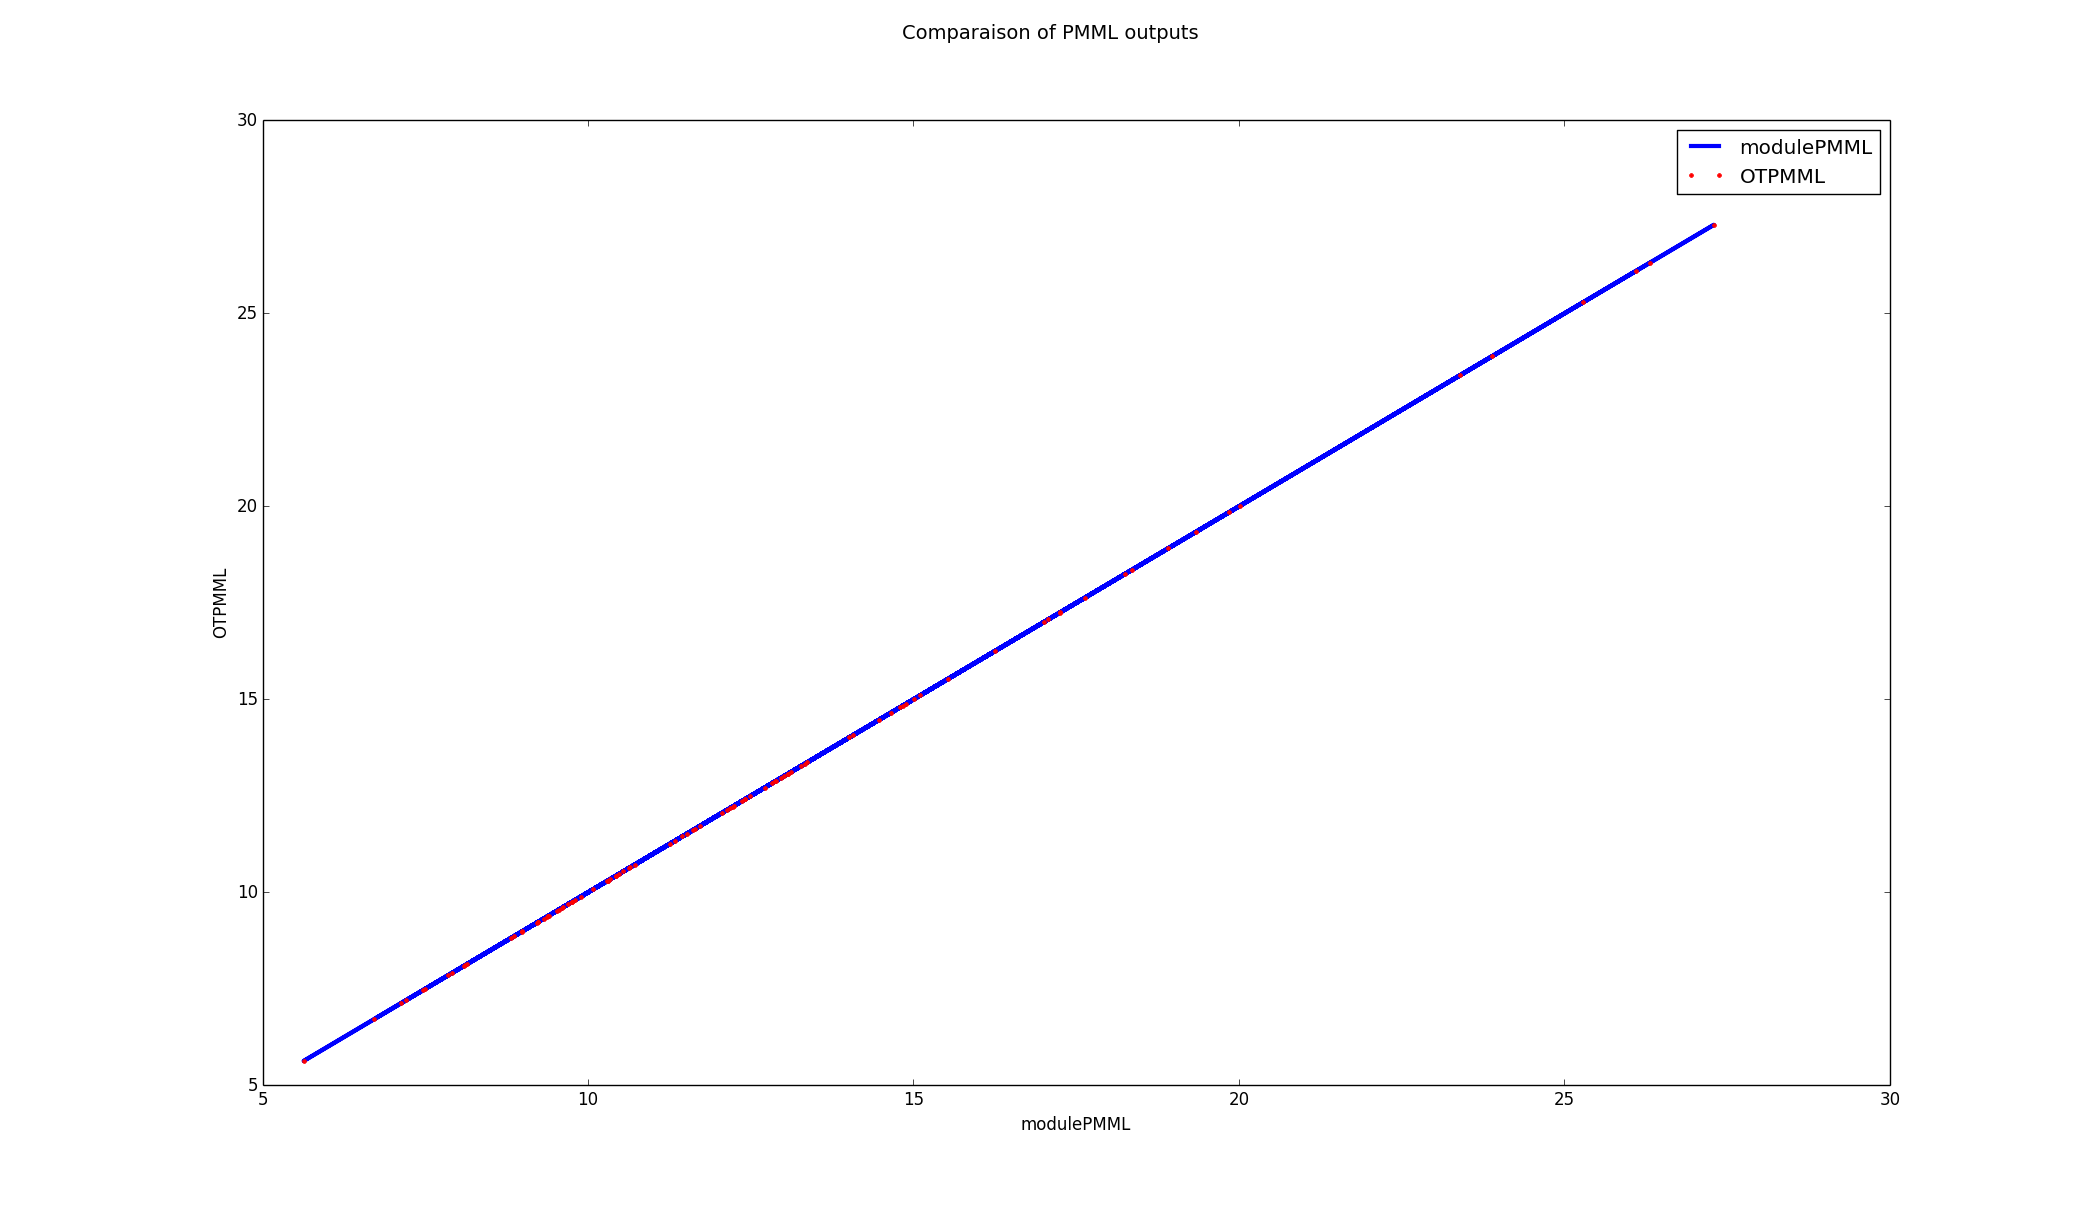
\includegraphics[scale=0.22]{comparaison_outputs.png}
 \end{center}
 \caption{Comparison of outputs}
 \label{fig:val:outputs}
\end{figure}
\newpage
In addition, errors are ploted in figure \ref{fig:val:errors}.
\begin{figure}[h]
 \begin{center}
  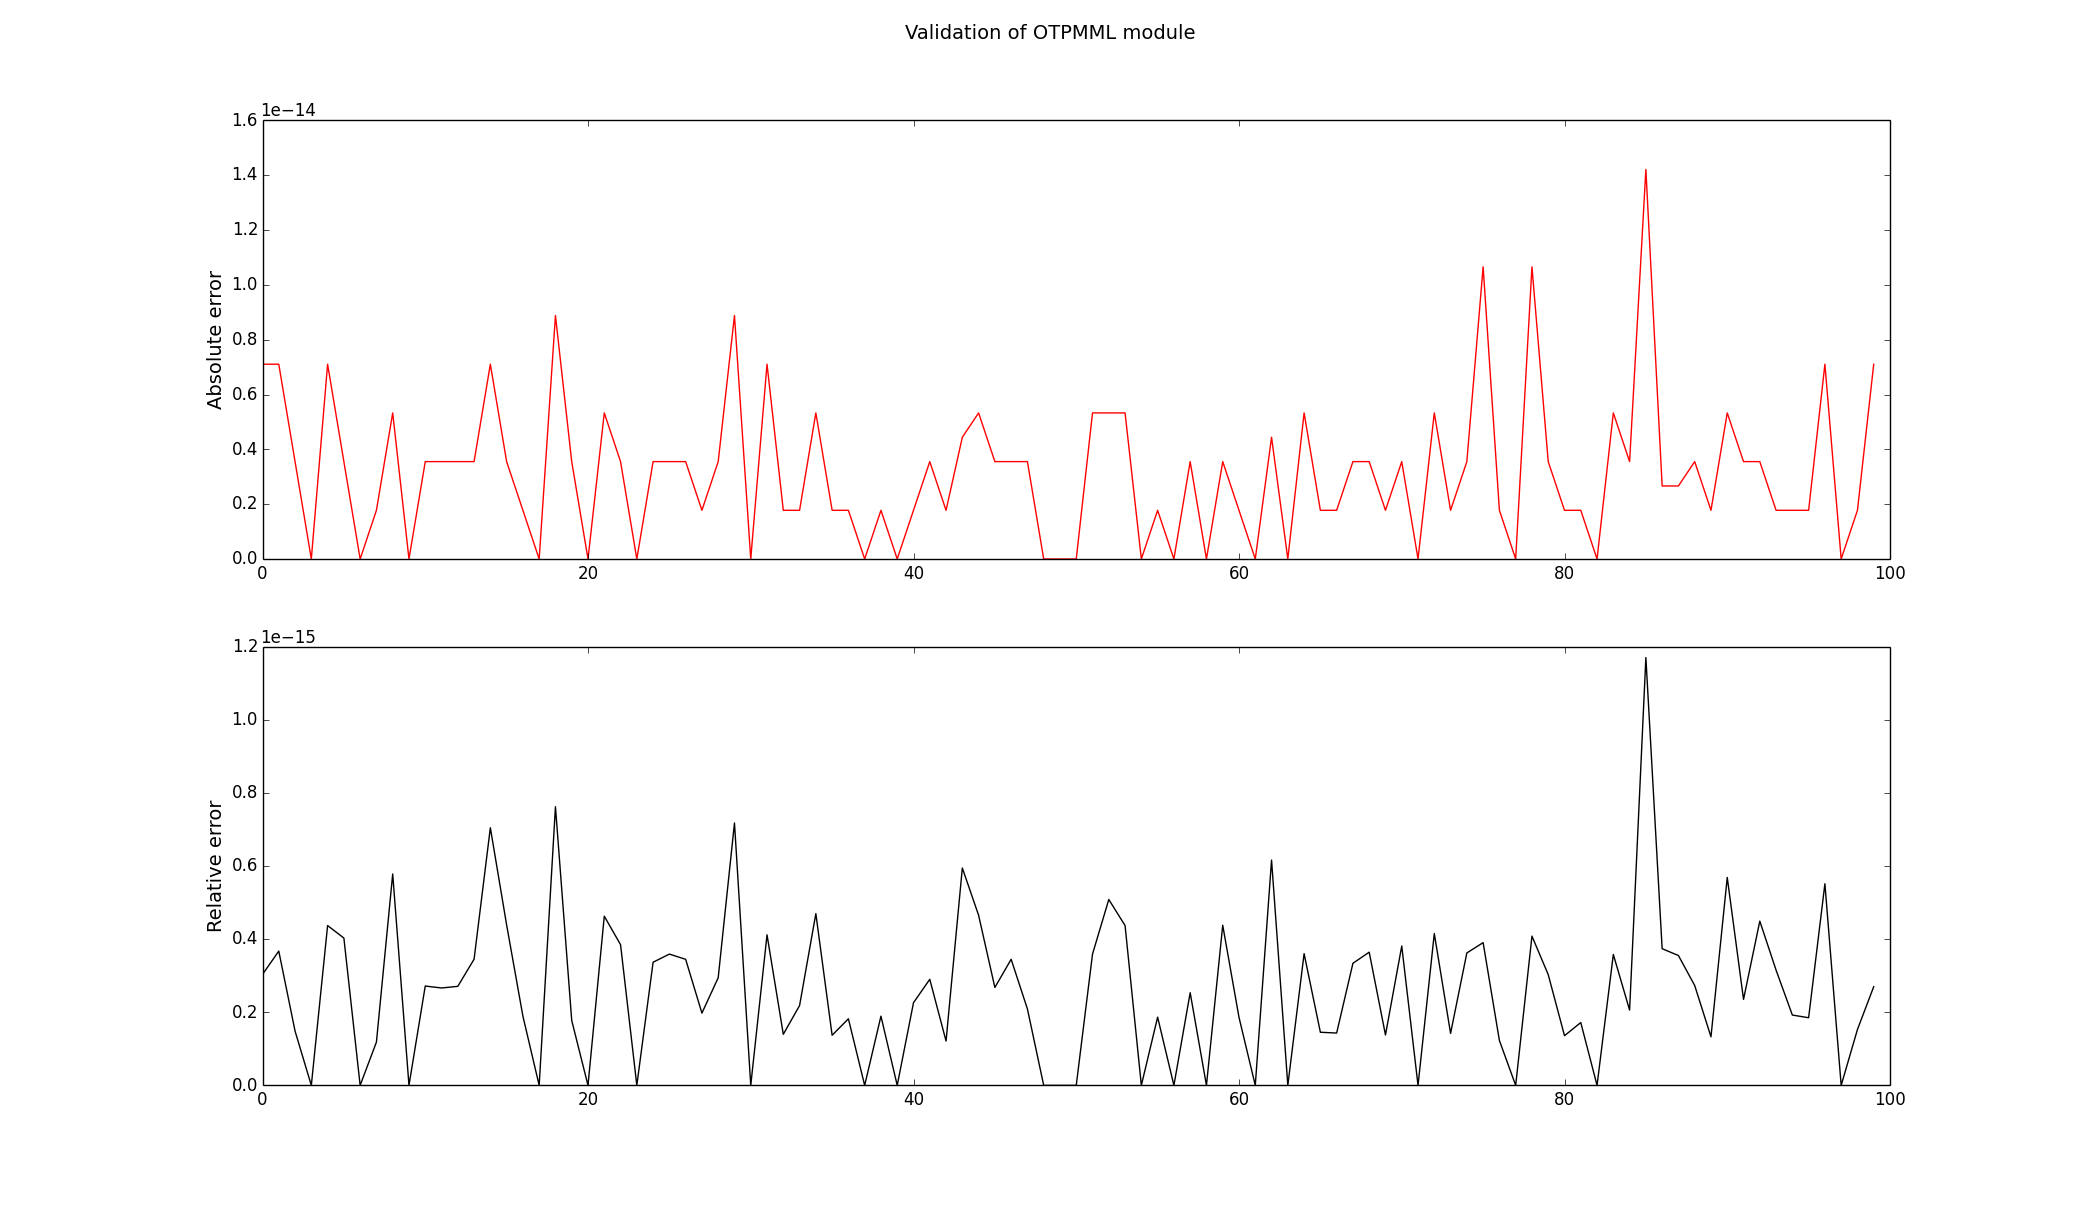
\includegraphics[scale=0.22]{absolute_relative_errors.png}
 \end{center}
 \caption{Comparison of outputs}
 \label{fig:val:errors}
\end{figure}
Comparisons are very good, absolute error is less than $1.5 \times 10^{-14}$ and relative errors less than $1.2 \times 10^{-15}$ , which validate the parsing.
\printindex
\end{document}
